% This file provides an example Beamer presentation using the RWTH theme
% showcasing some of the more common options, similar to the Powerpoint version
% 12.11.2014: Revision 1 (Harold Bruintjes, Tim Lange)

% For RWTH, beamer should be loaded with class option t (top)
\documentclass[t]{beamer} % use [handout] instead of [t] for handout

% Use fontspec to get Arial font
% Requires use of XeLaTeX
\usepackage{fontspec}
\setmainfont{Arial}
\setsansfont{Arial}
% Also force Arial for math for a more consistent look
\usepackage{unicode-math}

% https://tex.stackexchange.com/questions/426088/texlive-pretest-2018-beamer-and-subfig-collide
\makeatletter
\let\@@magyar@captionfix\relax
\makeatother

% German style date formatting (footer)
\usepackage[ddmmyyyy]{datetime}
\renewcommand{\dateseparator}{.}

\usepackage{MnSymbol,wasysym}

% Format the captions used for figures etc.
\usepackage[compatibility=false]{caption}
\captionsetup{singlelinecheck=off,justification=raggedleft,labelformat=empty,labelsep=none}

% PGFPlots is used for drawing some of the charts
\usepackage{pgfplots}
\pgfplotsset{compat=newest}
\input{plot_commands.tex}

% Load the actual RWTH theme. Suggested is to load the full theme,
% as it requires some specific dimensions
\usetheme{rwth}



% ---------------- My Stuff ---------------- %
% ---------- Hyperref ---------- %
\usepackage{hyperref}
\hypersetup{colorlinks,breaklinks,
            urlcolor=[rgb]{0,0.2,0.4},
            linkcolor=[rgb]{0,0.2,0.4}}
\def\UrlBreaks{\do\/\do-}
% Farbe ist darkmidnightblue
% ---------- -------- ---------- %
\usepackage{csquotes}

\begin{document}

\logo{\includegraphics{logo.png}}

% Setup presentation information
\title{Back-Propagation and Algorithms for Training Artificial Neural Networks with TensorFlow}
\date{30. October 2020}
\author{Gero Kauerauf}

\frame{\titlepage}

\section{List of Contents}
\begin{frame}
    \begin{figure}
        \centering
        \begin{itemize}[<+->]
            \item Introduction
            \item Data Representation
            \item AI Disciplines
            \item Neural Networks
            \item Linear Algebra
            \item Computational Graphs
            \item Back-Propagation
            \item Sources
        \end{itemize}
    \end{figure}
\end{frame}


\section{Introduction}
\begin{frame}
    \begin{itemize}[<+->]
        \item What is a complicated problem for a computer?
        \item A problems that is
        \begin{itemize}[<+->]
            \item hard to describe formally
            \item intuitive solvable for humans
        \end{itemize}
        \item For example: Recognizing a flower on a picture
        \item Deep Learning
        \begin{itemize}[<+->]
            \item Hierarchy of Concepts
            \item Representative Graph has Layers
        \end{itemize}
        \item Machine Learning
        \begin{itemize}[<+->]
            \item Acquiring its own knowledge
            \item Extracting patterns from data
        \end{itemize}
    \end{itemize}
\end{frame}

\section{Data Representation}
\begin{frame}
    \begin{itemize}[<+->]
        \item Importance of Data Representation
        \begin{itemize}[<+->]
            \item Tasks can be impossible in one representation and easy in another
            
            \begin{figure}
                \centering
                \begin{minipage}{0.45\textwidth}
                    \centering
                    \includegraphics[width=0.9\textwidth]{../plots/cartesian.pdf} % first figure itself
                \end{minipage}\hfill
                \begin{minipage}{0.45\textwidth}
                    \centering
                    \includegraphics[width=0.9\textwidth]{../plots/polar.pdf} % second figure itself
                \end{minipage}
            \end{figure}

            \item One solution to this is \textbf{representation learning}
            \begin{itemize}[<+->]
                \item Machine Learning now also discovers the representation itself
                \item Often better Performance
                \item AI can rapidly adapt to new tasks with minimal human intervention
            \end{itemize}
        \end{itemize}
    \end{itemize}
\end{frame}

\section{Different AI disciplines}
\begin{frame}
    \begin{itemize}
        \item Relations between different AI disciplines
        \begin{figure}
            %\centering
            \begin{minipage}{0.45\textwidth}
                \begin{figure}[]
                    \centering
                    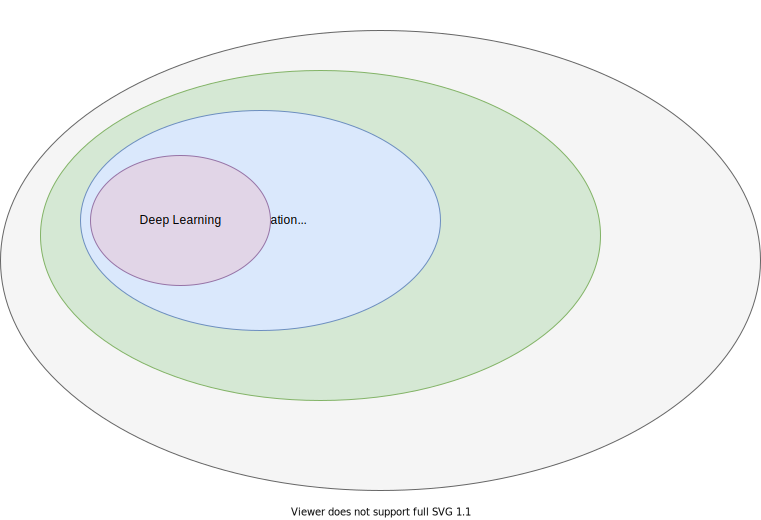
\includegraphics[width=\textwidth]{../plots/ai-venn.pdf}
                    %\caption{\href{http://www.deeplearningbook.org}{www.DeepLearningBook.org}}
                \end{figure}
            \end{minipage}\hfill
            \begin{minipage}{0.45\textwidth}
                \begin{figure}[]
                    \centering
                    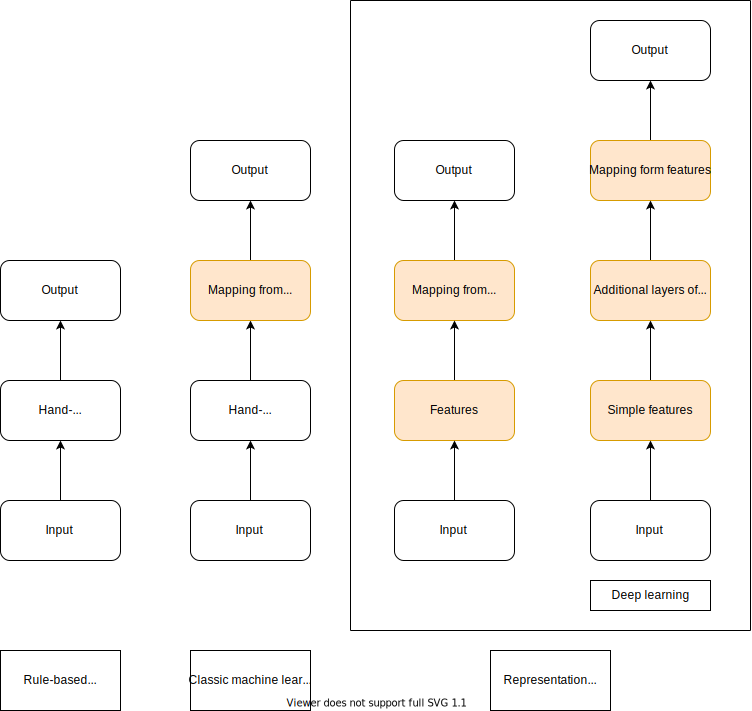
\includegraphics[width=\textwidth]{../plots/ai-flowchart.pdf}
                    %\caption{\href{http://www.deeplearningbook.org}{www.DeepLearningBook.org}}
                \end{figure}
            \end{minipage}
            \caption{\href{http://www.deeplearningbook.org}{www.DeepLearningBook.org}}
        \end{figure}
    \end{itemize}
\end{frame}

\section{Neural Networks}

\begin{frame}
    \begin{itemize}[<+->]
        \item An Neural Network consists out of nodes (vertices) and edges
        \item Nodes are modeling Neurons
        \item Edges are modeling synapses
        \item Nodes have an activations function (e.g. a rectifier function)
        \item The graph is weighted, that means each edge has a weight to it (\(w \in [0, 1]\))
    \end{itemize}

    \begin{itemize}[<+->]
        \item How it works:
        \begin{itemize}[<+->]
            \item Input nodes are given an input value
            \item Each node sums up the inputs that it gets and outputs the activation function value of that sum
        \end{itemize}
    \end{itemize}
\end{frame}

\begin{frame}
    \begin{figure}
        \centering
        \includegraphics[width=0.8\textwidth]{../plots/activation.pdf}   
    \end{figure}
    \begin{itemize}[<+->]
        \item Where \(x^T * w + b\) is nothing but \(\sum^{3}_{i=1}(x_i * w_i) + b\)
    \end{itemize}
\end{frame}

\begin{frame}
    \begin{itemize}[<+->]
        \item A deep neural network consists out of
        \begin{itemize}[<+->]
            \item an input layer
            \item multiple hidden layers
            \item an output layer
        \end{itemize}
        \begin{figure}
            \centering
            \includegraphics[width=0.9\textwidth]{../plots/nn-2-crop.pdf}
        \end{figure}
    \end{itemize}
\end{frame}

\section{Linear Algebra}
\begin{frame}
    \begin{itemize}[<+->]
        \item Nothing but linear algebra
        \item All operations can easily be described with vectors and matrices \\
        \item We can describe the weights of each layer of the DNN with a weight matrix
        \item The input can be written as a vector, same goes for the biases
        \item Thus propagating through the network is simply a matrix-vector multiplication plus the corresponding bias foreach layer
    \end{itemize}
\end{frame}

\section{Computational Graphs}
\begin{frame}
    \begin{figure}
        \centering
        \begin{minipage}{0.45\textwidth}
            \begin{figure}[]
                \centering
                \includegraphics[width=0.5\textwidth]{../plots/computational-graph-c-crop.pdf}
            \end{figure}
        \end{minipage}\hfill
        \begin{minipage}{0.45\textwidth}
            \centering
            \begin{figure}[]
                \includegraphics[width=0.45\textwidth]{../plots/computational-graph-b-crop.pdf}
            \end{figure}
        \end{minipage}
        \caption{\href{http://www.deeplearningbook.org}{www.DeepLearningBook.org}}
    \end{figure}
    \begin{itemize}[<+->]
        \item A computational graph is used to describe a mathematical expression as a graph
        \item This allows us to apply \emph{graph algorithms} on it
    \end{itemize}
\end{frame}

\begin{frame}
    \begin{figure}
        \centering
        \begin{minipage}{0.45\textwidth}
            \begin{figure}[]
                \centering
                \includegraphics[width=0.7\textwidth]{../plots/computational-graph-c-crop.pdf}
            \end{figure}
        \end{minipage}\hfill
        \begin{minipage}{0.45\textwidth}
            \begin{itemize}[<+->]
                \item First we compute \(XW\), that we store in \(U^{(1)}\)
                \item Then we calculate \(U^{(2)} = U^{(1)} + b \; \Leftrightarrow \; U^{(2)} = XW + b\)
                \item Finally ReLU refers to \emph{rectifier linear unit}
                \item \(\rightarrow f(x) = max\{0, x\} = \vert x\vert\) \\
                \item This computational graph computes \(H = max\{0, XW + b\}\)
            \end{itemize}
        \end{minipage}
        \caption{\href{http://www.deeplearningbook.org}{www.DeepLearningBook.org}}
    \end{figure}
\end{frame}

\begin{frame}
    \begin{figure}
        \centering
        \begin{minipage}{0.45\textwidth}
            \begin{itemize}[<+->]
                \item This one here computes \(\hat{y} = \sigma (x^T w + b)\)
            \end{itemize}
        \end{minipage}\hfill
        \begin{minipage}{0.45\textwidth}
            \centering
            \begin{figure}[]
                \includegraphics[width=0.6\textwidth]{../plots/computational-graph-b-crop.pdf}
            \end{figure}
        \end{minipage}
    \end{figure}
\end{frame}

\section{Back-Propagation}
\begin{frame}
    \begin{itemize}[<+->]
        \item Back-Propagation is a \enquote{graph algorithm} that we can use to compute the the gradient of a graph
        \item Backpropagation is the recursive usage of the \emph{Chain-Rule} to obtain the gradient \\
        \item We can now define a cost function for a DNN
        \item For that cost function we can find the respective computational graph
        \item We can use the Back-Propagation to find the gradient of the cost function
        \item And then find the minimum of the gradient of the cost function via \emph{Stochastic Gradient Descent} (SGD) an extension of the normal \emph{Gradient Descent}, which is an iterative algorithm for finding a local minimum
    \end{itemize}
\end{frame}

\section{Sources}
\begin{frame}
    \begin{itemize}[<+->]
        \item Sources:
        \begin{itemize}[<+->]
            \item \textbf{Deep Learning} by Ian Goodfellow and Yoshua Bengio and Aaron Courville \\
            \href{https://www.deeplearningbook.org}{www.deeplearningbook.org}
            \item \textbf{TensorFlow} \\
            \href{https://www.tensorflow.org}{www.tensorflow.org} \\

            \item And of course wikipedia for quick look ups
        \end{itemize}
        \item Tools used:
        \begin{itemize}[<+->]
            \item \textbf{Graphviz} for plotting computational graphs \\
            \href{https://graphviz.org}{www.graphviz.org}
            \item \textbf{matplotlib} for more plots \\
            \href{https://matplotlib.org}{www.matplotlib.org}
        \end{itemize}
    \end{itemize}
\end{frame}

\end{document}